% =====================================================================
% Template Laporan Tugas — Workshop Deep Learning (Teknik Telekomunikasi ITERA)
% Studi Ablasi RNN, LSTM, GRU vs ANN untuk Prediksi Trafik Seluler
%
% Format IEEE conference dua kolom, MAKSIMAL 6 HALAMAN termasuk referensi.
% Compile: pdflatex main && bibtex main && pdflatex main && pdflatex main
%          (atau: latexmk -pdf main.tex). Bisa juga diunggah ke Overleaf.
%
% Teks bertanda [ ... ] adalah petunjuk: HAPUS dan ganti dengan isi kalian.
% =====================================================================
\documentclass[conference,a4paper]{IEEEtran}
\IEEEoverridecommandlockouts

\usepackage[indonesian]{babel}
\usepackage[utf8]{inputenc}
\usepackage[T1]{fontenc}
\usepackage{cite}
\usepackage{amsmath,amssymb}
\usepackage{graphicx}
\usepackage{booktabs}
\usepackage{siunitx}
\usepackage{xcolor}
\usepackage[hidelinks]{hyperref}
\graphicspath{{gambar/}}

% Penanda petunjuk (hapus pemakaiannya di versi akhir)
\newcommand{\petunjuk}[1]{\textcolor{gray}{[#1]}}

\begin{document}

\title{Studi Ablasi RNN, LSTM, dan GRU dibandingkan ANN untuk Prediksi Trafik Seluler Kota Milan}

% Satu blok per anggota (maks. 3). Hapus blok yang tidak dipakai.
\author{
\IEEEauthorblockN{Andryansyah Amir}
\IEEEauthorblockA{NIM 124400065\\
Teknik Telekomunikasi, ITERA\\
andryansyah.124400065@student.itera.ac.id}
\and
\IEEEauthorblockN{Ade Raka Maulana}
\IEEEauthorblockA{NIM 124400047\\
Teknik Telekomunikasi, ITERA\\
ade.124400047@student.itera.ac.id}
}

\maketitle

\begin{abstract}
Prakiraan trafik internet per jam pada tingkat sel membantu operator seluler merencanakan kapasitas jaringan. Studi ini membandingkan ANN, RNN, LSTM, dan GRU pada data Telecom Italia di kotak Duomo, Milan, dan menguji generalisasinya di Bandara Linate. Dengan studi ablasi, lima faktor wajib (panjang jendela, ukuran hidden, jumlah lapisan, \textit{learning rate}, dan kelompok fitur) serta tiga faktor pilihan (\textit{optimizer}, fungsi \textit{loss}, dan \textit{patience}) diubah satu per satu dari konfigurasi acuan, masing-masing dengan tiga seed. Pada acuan, RNN dan GRU mencapai test MAE $229{,}6 \pm 5{,}1$ dan $237{,}2 \pm 9{,}3$, jauh di bawah ANN ($309{,}9 \pm 5{,}9$) dan baseline naif terbaik ($467{,}6$). ANN paling sensitif terhadap panjang jendela (val MAE $211{,}5$ menjadi $298{,}2$ saat $W$ naik dari 6 ke 168 jam), sedangkan GRU paling diuntungkan oleh ukuran hidden besar (val MAE $188{,}7$ pada hidden 128 dibanding $207{,}5$ pada acuan). \textit{Learning rate} $10^{-4}$ dan SGD gagal konvergen dalam 300 epoch. \petunjuk{Satu kalimat tentang konfigurasi terbaik dan hasil di Linate: isi setelah Bagian C dan D selesai.} Hasil menunjukkan bahwa model rekuren lebih akurat dan lebih tahan terhadap pilihan hyperparameter daripada ANN pada data ini.
\end{abstract}

\begin{IEEEkeywords}
prediksi trafik seluler, RNN, LSTM, GRU, studi ablasi
\end{IEEEkeywords}

% ---------------------------------------------------------------------
\section{Pendahuluan}
Prakiraan trafik per sel membantu operator seluler merencanakan kapasitas, menghemat energi pada jam sepi, dan mendeteksi lonjakan yang tidak biasa. Trafik per jam memiliki pola harian dan mingguan yang kuat, sehingga model sekuensial seperti RNN, LSTM \cite{hochreiter1997lstm}, dan GRU \cite{cho2014gru} diharapkan lebih unggul daripada ANN yang memperlakukan jendela masukan sebagai vektor datar. Namun, membandingkan model pada satu konfigurasi saja dapat menyesatkan karena hasilnya bergantung pada pilihan hyperparameter. Studi ablasi mengubah satu faktor dalam satu waktu dari konfigurasi acuan, sehingga pengaruh tiap faktor dapat dipisahkan. Kontribusi laporan ini:
\begin{itemize}\setlength{\itemsep}{0pt}
  \item ablasi delapan faktor (lima wajib, tiga pilihan) pada empat model dengan tiga seed;
  \item perbandingan konfigurasi terbaik dengan acuan dan baseline naif pada minggu test dan Natal;
  \item uji generalisasi konfigurasi terbaik di lokasi kelompok.
\end{itemize}

% ---------------------------------------------------------------------
\section{Data dan Metode}

\subsection{Dataset}
Data berasal dari Telecom Italia Big Data Challenge \cite{barlacchi2015milan}, yang dipakai dalam versi agregat per jam dari \cite{zhang2021fedda}, mencakup November--Desember 2013 dengan resolusi satu jam. Setiap kotak grid Milan memiliki tiga deret waktu: aktivitas internet (\textit{net}, yang menjadi target prediksi), panggilan (\textit{call}), dan SMS (\textit{sms}). Dua fitur waktu ditambahkan, yaitu jam dan hari dalam seminggu, masing-masing dikodekan sebagai sinus dan kosinus, sehingga total tujuh fitur. Lokasi utama adalah kotak Duomo (5060). Lokasi kelompok adalah kode 5, Bandara Linate (kotak 4489); posisi lokasi tugas ditunjukkan pada Gambar~\ref{fig:peta}.

\begin{figure}[t]
  \centering
  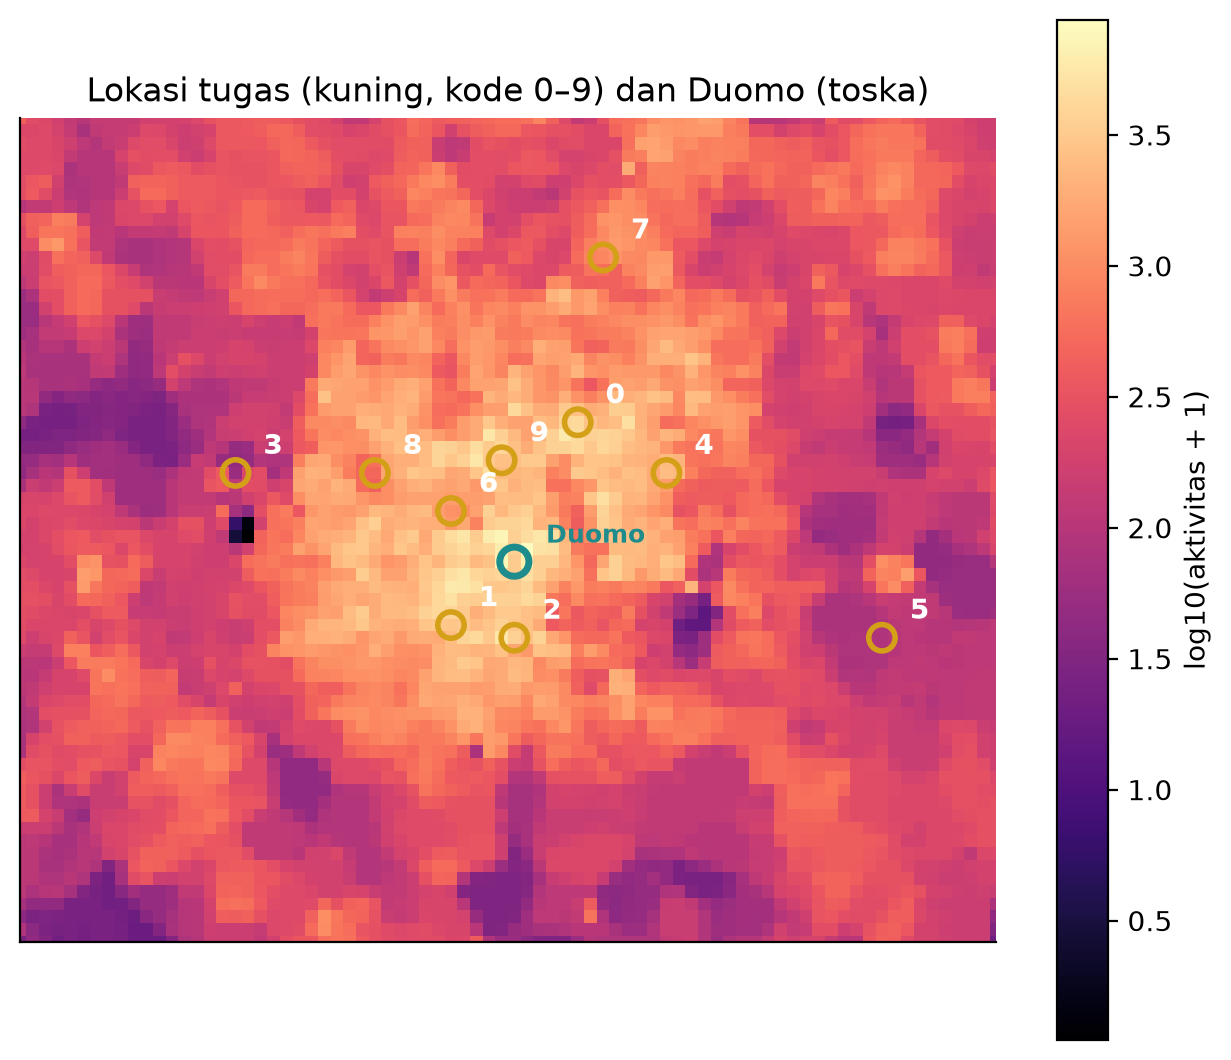
\includegraphics[width=0.85\linewidth]{peta_lokasi_tugas.png}
  \caption{Rata-rata aktivitas internet per kotak di Milan. Lingkaran kuning: lokasi tugas (kode 0--9); lingkaran toska: Duomo.}
  \label{fig:peta}
\end{figure}

\subsection{Pembagian Data dan Praproses}
Data dibagi berdasarkan waktu: latih 11 November--8 Desember (28 hari, 672 sampel), validasi 9--15 Desember, test 16--22 Desember, dan minggu Natal 23--29 Desember 2013. Minggu 4--10 November hanya menjadi konteks untuk jendela awal. Data deret waktu tidak boleh diacak karena sampel yang berdekatan saling berkorelasi; pengacakan membuat model melihat masa depan saat berlatih sehingga galat tampak lebih kecil daripada yang akan terjadi ketika model benar-benar meramal. Standarisasi memakai rata-rata dan simpangan baku dari data sebelum minggu validasi saja, agar tidak ada informasi validasi dan test yang bocor ke pelatihan. Pada \textit{windowing}, setiap sampel berupa jendela $W$ jam terakhir sebagai masukan dan nilai \textit{net} jam berikutnya sebagai target (horizon 1).

\subsection{Model dan Konfigurasi Acuan}
ANN meratakan jendela masukan $[W, \text{fitur}]$ menjadi satu vektor, melewatkannya ke sejumlah lapisan tersembunyi dengan aktivasi ReLU, lalu satu lapisan keluaran. RNN, LSTM, dan GRU menumpuk lapisan rekuren dan mengambil \textit{hidden state} pada jam terakhir, yang kemudian dipetakan ke keluaran dengan satu lapisan linear. LSTM dan GRU menambahkan gerbang pada sel rekuren untuk mengatur informasi yang disimpan dan dilupakan. Seluruh model diimplementasikan dengan PyTorch \cite{paszke2019pytorch}. Ukuran hidden acuan dipilih agar jumlah parameter model rekuren sekitar 5,5 ribu (RNN 5.305, LSTM 5.578, GRU 5.397; ANN 6.497), sehingga perbandingan pada acuan relatif adil dalam kapasitas (Tabel~\ref{tab:acuan}).

\begin{table}[t]
  \centering
  \caption{Konfigurasi acuan}
  \label{tab:acuan}
  \begin{tabular}{@{}ll@{}}
    \toprule
    Hyperparameter & Nilai acuan \\
    \midrule
    Panjang jendela $W$ & 24 jam \\
    Horizon & 1 jam \\
    Ukuran hidden & ANN 32, RNN 68, LSTM 33, GRU 38 \\
    Jumlah lapisan & ANN 2, rekuren 1 \\
    Fitur & net, call, sms, jam, hari (7) \\
    Optimizer, \textit{learning rate} & Adam, $10^{-3}$ \\
    \textit{Batch size} & 64 \\
    \textit{Early stopping} & \textit{patience} 30, maks.\ 300 epoch \\
    \bottomrule
  \end{tabular}
\end{table}

\subsection{Protokol Ablasi dan Evaluasi}
Satu faktor diubah setiap kali, faktor lain tetap pada acuan. Faktor wajib: A1 panjang jendela $W \in \{6, 12, 24, 48, 168\}$ jam, A2 ukuran hidden $\{16, 32, 64, 128\}$, A3 jumlah lapisan $\{1, 2, 3\}$, A4 \textit{learning rate} $\{10^{-4}, 10^{-3}, 10^{-2}\}$, dan A5 kelompok fitur (net; net+call+sms; net+waktu; semua). Faktor pilihan: B3 \textit{optimizer} (Adam, AdamW, SGD), B4 fungsi \textit{loss} (MSE, MAE, Huber), dan B5 \textit{patience} $\{10, 30, 60\}$. Hipotesis awal: \petunjuk{tulis hipotesis kelompokmu untuk B3, B4, B5 sebelum melihat hasil}. Setiap konfigurasi dilatih dengan tiga seed (0, 1, 2) dan dilaporkan sebagai rata-rata $\pm$ simpangan baku. Metrik adalah MAE, RMSE, dan MAPE pada skala asli (bukan skala terstandarisasi). \textit{Early stopping} memakai MSE validasi dan memulihkan bobot terbaik. Konfigurasi terbaik dipilih berdasarkan val MAE, sedangkan minggu test dan Natal hanya dipakai untuk pelaporan. Seluruh pelatihan berjalan di CPU dengan PyTorch 2.14.1, dengan total waktu pelatihan 71,3 menit.

% ---------------------------------------------------------------------
\section{Hasil}

\subsection{Baseline Naif dan Acuan}
Tabel~\ref{tab:naif} memuat tiga tebakan naif (nilai terakhir, jam yang sama kemarin, dan jam yang sama minggu lalu) serta hasil konfigurasi acuan. Pada minggu test, baseline naif terbaik adalah ``minggu lalu'' dengan MAE $467{,}6$. Semua model acuan mengungguli angka ini: RNN ($229{,}6$) dan GRU ($237{,}2$) sekitar dua kali lebih baik, sedangkan LSTM ($273{,}6$) dan ANN ($309{,}9$) sekitar $1{,}5$--$1{,}7$ kali lebih baik. Di antara model, RNN paling akurat dan ANN paling lemah; selisih RNN dan GRU lebih kecil daripada simpangan baku GRU ($9{,}3$), sehingga keduanya belum dapat dibedakan. Pada minggu Natal, urutan baseline berubah: tebakan ``minggu lalu'' memburuk drastis ($1426{,}2$) karena pola Natal berbeda dari minggu biasa, sedangkan ``nilai terakhir'' ($431{,}2$) menjadi baseline terbaik. Hanya RNN ($421{,}2 \pm 2{,}4$) yang berada di bawah angka tersebut; ANN, LSTM, dan GRU lebih buruk.

\begin{table}[t]
  \centering
  \caption{MAE baseline naif dan konfigurasi acuan di Duomo (model: rata-rata $\pm$ simpangan baku, 3 seed).}
  \label{tab:naif}
  \footnotesize
  \setlength{\tabcolsep}{3pt}
  \begin{tabular}{@{}lccc@{}}
    \toprule
    Metode & Val & Test & Natal \\
    \midrule
    Naif: terakhir    & 662,6 & 600,9 & 431,2 \\
    Naif: kemarin     & 595,3 & 552,2 & 921,5 \\
    Naif: minggu lalu & 492,8 & 467,6 & 1426,2 \\
    \midrule
    ANN  & $248{,}9 \pm 8{,}9$  & $309{,}9 \pm 5{,}9$  & $680{,}1 \pm 52{,}0$ \\
    RNN  & $206{,}1 \pm 7{,}4$  & $229{,}6 \pm 5{,}1$  & $421{,}2 \pm 2{,}4$ \\
    LSTM & $230{,}5 \pm 12{,}2$ & $273{,}6 \pm 25{,}4$ & $586{,}0 \pm 56{,}8$ \\
    GRU  & $207{,}5 \pm 3{,}8$  & $237{,}2 \pm 9{,}3$  & $468{,}2 \pm 21{,}8$ \\
    \bottomrule
  \end{tabular}
\end{table}

\subsection{Ablasi Wajib}
Tabel~\ref{tab:ablasi} merangkum seluruh ablasi dalam val MAE, nilai yang dipakai untuk memilih konfigurasi; faktor A1--A5 dibahas di bawah dan faktor B di subbagian berikutnya.

\begin{table*}[t]
  \centering
  \caption{Ablasi faktor tunggal di Duomo: val MAE (rata-rata $\pm$ simpangan baku, 3 seed). Cetak tebal: nilai terbaik tiap model dalam satu faktor. Fitur: n+c+s = net+call+sms; n+waktu = net+jam+hari.}
  \label{tab:ablasi}
  \footnotesize
  \setlength{\tabcolsep}{3pt}
  \begin{minipage}[t]{0.49\textwidth}
    \centering
    \begin{tabular}{@{}lcccc@{}}
      \toprule
      Faktor / nilai & ANN & RNN & LSTM & GRU \\
      \midrule
      \multicolumn{5}{@{}l}{\textit{A1: panjang jendela $W$ (jam)}} \\
      6   & $\mathbf{211{,}5} \pm 6{,}2$ & $215{,}5 \pm 4{,}1$  & $\mathbf{227{,}1} \pm 4{,}3$ & $212{,}6 \pm 11{,}5$ \\
      12  & $238{,}5 \pm 4{,}5$  & $206{,}7 \pm 6{,}2$  & $235{,}6 \pm 2{,}0$  & $208{,}9 \pm 10{,}4$ \\
      24  & $248{,}9 \pm 8{,}9$  & $206{,}1 \pm 7{,}4$  & $230{,}5 \pm 12{,}2$ & $207{,}5 \pm 3{,}8$ \\
      48  & $262{,}6 \pm 3{,}8$  & $\mathbf{200{,}1} \pm 5{,}3$ & $249{,}1 \pm 21{,}8$ & $\mathbf{206{,}7} \pm 5{,}0$ \\
      168 & $298{,}2 \pm 18{,}2$ & $204{,}8 \pm 10{,}2$ & $241{,}4 \pm 8{,}1$  & $\mathbf{206{,}7} \pm 5{,}1$ \\
      \midrule
      \multicolumn{5}{@{}l}{\textit{A2: ukuran hidden}} \\
      16  & $257{,}6 \pm 28{,}0$ & $247{,}0 \pm 5{,}8$  & $244{,}3 \pm 18{,}3$ & $216{,}8 \pm 21{,}2$ \\
      32  & $248{,}9 \pm 8{,}9$  & $218{,}7 \pm 6{,}6$  & $241{,}5 \pm 20{,}5$ & $210{,}2 \pm 0{,}8$ \\
      64  & $238{,}4 \pm 16{,}5$ & $\mathbf{207{,}2} \pm 12{,}8$ & $218{,}1 \pm 1{,}9$ & $198{,}4 \pm 9{,}2$ \\
      128 & $\mathbf{233{,}8} \pm 1{,}9$ & $207{,}7 \pm 7{,}2$ & $\mathbf{207{,}1} \pm 8{,}4$ & $\mathbf{188{,}7} \pm 4{,}2$ \\
      \midrule
      \multicolumn{5}{@{}l}{\textit{A3: jumlah lapisan}} \\
      1 & $\mathbf{240{,}9} \pm 7{,}5$ & $\mathbf{206{,}1} \pm 7{,}4$ & $\mathbf{230{,}5} \pm 12{,}2$ & $207{,}5 \pm 3{,}8$ \\
      2 & $248{,}9 \pm 8{,}9$  & $207{,}3 \pm 9{,}1$  & $254{,}8 \pm 14{,}5$ & $\mathbf{203{,}3} \pm 9{,}6$ \\
      3 & $249{,}3 \pm 11{,}7$ & $225{,}1 \pm 12{,}7$ & $338{,}9 \pm 16{,}9$ & $212{,}2 \pm 15{,}9$ \\
      \midrule
      \multicolumn{5}{@{}l}{\textit{A4: \textit{learning rate}}} \\
      $10^{-4}$ & $295{,}4 \pm 4{,}7$  & $285{,}0 \pm 13{,}7$ & $399{,}4 \pm 25{,}0$ & $398{,}4 \pm 8{,}6$ \\
      $10^{-3}$ & $\mathbf{248{,}9} \pm 8{,}9$ & $\mathbf{206{,}1} \pm 7{,}4$ & $230{,}5 \pm 12{,}2$ & $\mathbf{207{,}5} \pm 3{,}8$ \\
      $10^{-2}$ & $261{,}8 \pm 16{,}6$ & $227{,}2 \pm 6{,}4$  & $\mathbf{215{,}9} \pm 14{,}2$ & $208{,}2 \pm 5{,}6$ \\
      \bottomrule
    \end{tabular}
  \end{minipage}\hfill
  \begin{minipage}[t]{0.49\textwidth}
    \centering
    \begin{tabular}{@{}lcccc@{}}
      \toprule
      Faktor / nilai & ANN & RNN & LSTM & GRU \\
      \midrule
      \multicolumn{5}{@{}l}{\textit{A5: kelompok fitur}} \\
      net     & $260{,}5 \pm 7{,}0$  & $245{,}2 \pm 5{,}8$  & $266{,}2 \pm 5{,}7$  & $264{,}6 \pm 7{,}0$ \\
      n+c+s   & $259{,}9 \pm 5{,}2$  & $224{,}1 \pm 2{,}3$  & $243{,}7 \pm 7{,}1$  & $231{,}8 \pm 12{,}6$ \\
      n+waktu & $\mathbf{246{,}0} \pm 9{,}8$ & $223{,}0 \pm 9{,}5$ & $231{,}1 \pm 4{,}3$ & $213{,}2 \pm 18{,}2$ \\
      semua   & $248{,}9 \pm 8{,}9$  & $\mathbf{206{,}1} \pm 7{,}4$ & $\mathbf{230{,}5} \pm 12{,}2$ & $\mathbf{207{,}5} \pm 3{,}8$ \\
      \midrule
      \multicolumn{5}{@{}l}{\textit{B3: \textit{optimizer}}} \\
      adam  & $248{,}9 \pm 8{,}9$  & $\mathbf{206{,}1} \pm 7{,}4$ & $\mathbf{230{,}5} \pm 12{,}2$ & $\mathbf{207{,}5} \pm 3{,}8$ \\
      adamw & $\mathbf{246{,}3} \pm 11{,}9$ & $\mathbf{206{,}1} \pm 7{,}4$ & $\mathbf{230{,}5} \pm 12{,}2$ & $\mathbf{207{,}5} \pm 3{,}8$ \\
      sgd   & $279{,}2 \pm 12{,}4$ & $299{,}2 \pm 10{,}2$ & $413{,}6 \pm 14{,}3$ & $371{,}2 \pm 2{,}0$ \\
      \midrule
      \multicolumn{5}{@{}l}{\textit{B4: fungsi \textit{loss}}} \\
      mse   & $248{,}9 \pm 8{,}9$  & $\mathbf{206{,}1} \pm 7{,}4$ & $\mathbf{230{,}5} \pm 12{,}2$ & $\mathbf{207{,}5} \pm 3{,}8$ \\
      mae   & $\mathbf{238{,}4} \pm 5{,}3$ & $217{,}9 \pm 9{,}3$ & $239{,}2 \pm 9{,}6$ & $213{,}5 \pm 14{,}7$ \\
      huber & $241{,}9 \pm 3{,}7$  & $206{,}3 \pm 10{,}0$ & $233{,}6 \pm 13{,}6$ & $207{,}8 \pm 5{,}1$ \\
      \midrule
      \multicolumn{5}{@{}l}{\textit{B5: \textit{patience}}} \\
      10 & $271{,}8 \pm 23{,}2$ & $220{,}2 \pm 11{,}4$ & $250{,}1 \pm 2{,}5$ & $218{,}1 \pm 4{,}8$ \\
      30 & $248{,}9 \pm 8{,}9$  & $\mathbf{206{,}1} \pm 7{,}4$ & $230{,}5 \pm 12{,}2$ & $207{,}5 \pm 3{,}8$ \\
      60 & $\mathbf{241{,}8} \pm 3{,}8$ & $206{,}6 \pm 7{,}0$ & $\mathbf{223{,}3} \pm 7{,}6$ & $\mathbf{205{,}6} \pm 9{,}9$ \\
      \bottomrule
    \end{tabular}
  \end{minipage}
\end{table*}

\begin{figure*}[t]
  \centering
  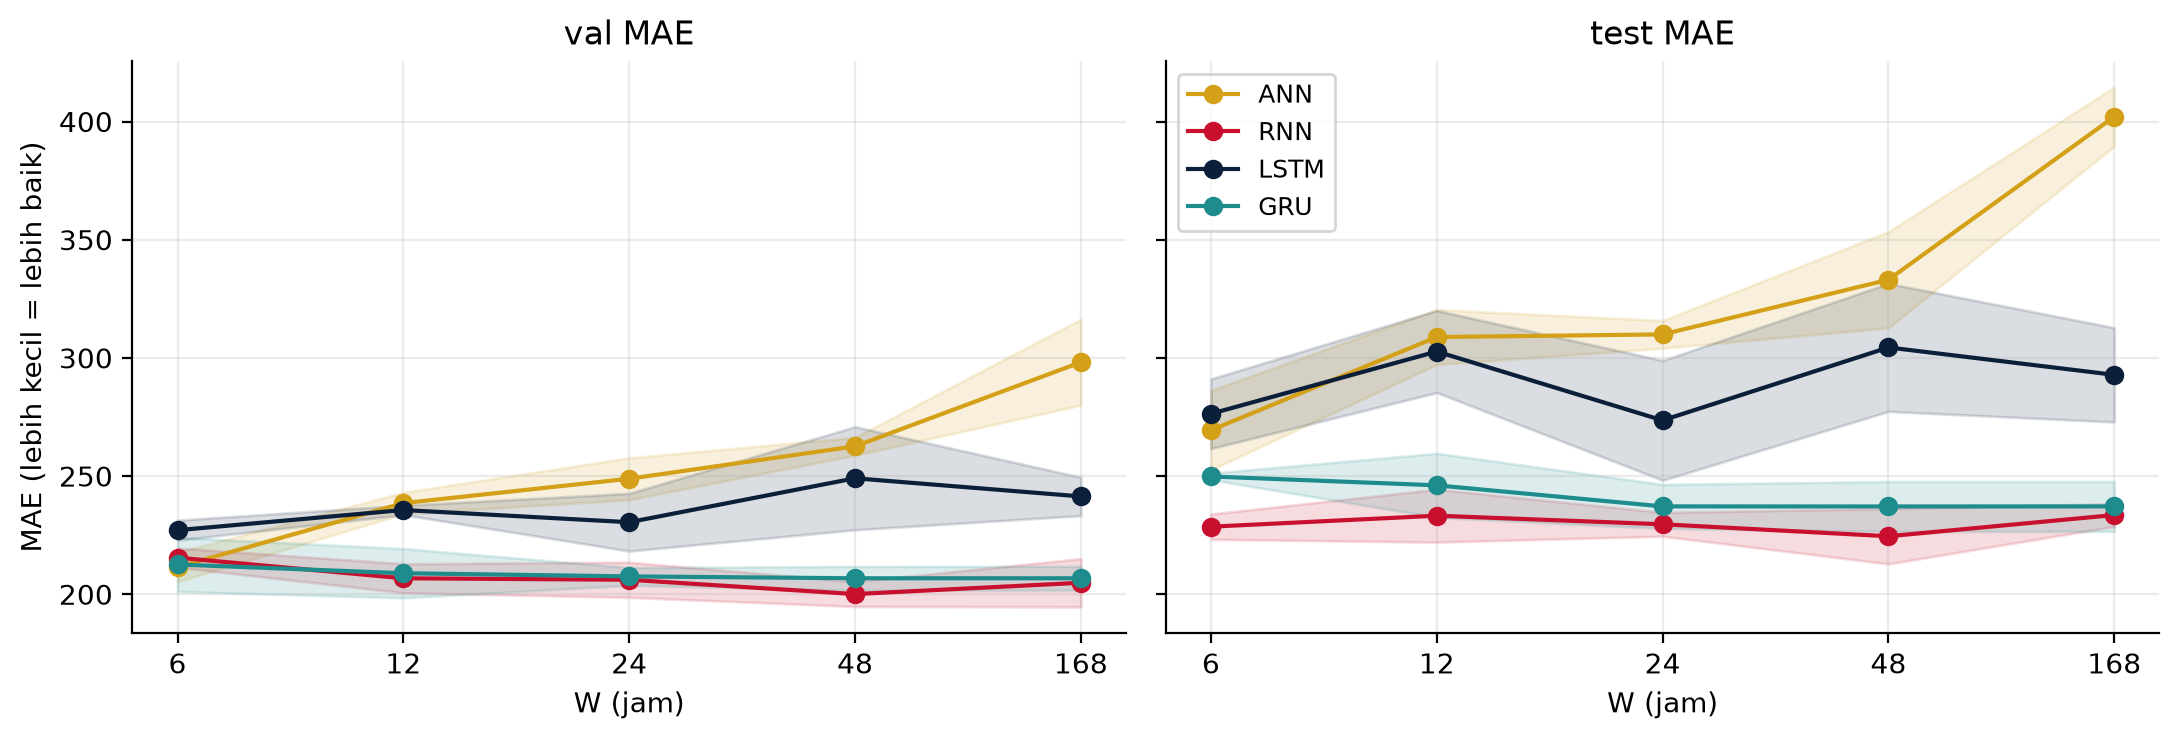
\includegraphics[width=0.8\textwidth]{A1_W.png}
  \caption{Pengaruh panjang jendela $W$ terhadap MAE validasi (kiri) dan test (kanan) di Duomo. Garis: rata-rata tiga seed; area: $\pm 1$ simpangan baku.}
  \label{fig:a1}
\end{figure*}

\begin{table}[t]
  \centering
  \caption{Pengaruh panjang jendela $W$ terhadap test MAE di Duomo (rata-rata $\pm$ simpangan baku, 3 seed). Cetak tebal: test MAE terendah tiap model; pemilihan konfigurasi tetap memakai val MAE (Tabel~\ref{tab:ablasi}).}
  \label{tab:a1test}
  \footnotesize
  \setlength{\tabcolsep}{3pt}
  \begin{tabular}{@{}lcccc@{}}
    \toprule
    $W$ (jam) & ANN & RNN & LSTM & GRU \\
    \midrule
    6   & $\mathbf{269{,}4 \pm 16{,}8}$ & $228{,}6 \pm 5{,}4$  & $276{,}3 \pm 14{,}7$ & $249{,}8 \pm 1{,}4$ \\
    12  & $308{,}8 \pm 11{,}6$ & $233{,}2 \pm 11{,}2$ & $302{,}7 \pm 17{,}4$ & $246{,}1 \pm 13{,}5$ \\
    24  & $309{,}9 \pm 5{,}9$  & $229{,}6 \pm 5{,}1$  & $\mathbf{273{,}6 \pm 25{,}4}$ & $237{,}2 \pm 9{,}3$ \\
    48  & $333{,}1 \pm 20{,}3$ & $\mathbf{224{,}5 \pm 11{,}7}$ & $304{,}4 \pm 27{,}1$ & $\mathbf{237{,}1 \pm 10{,}6}$ \\
    168 & $402{,}0 \pm 12{,}5$ & $233{,}5 \pm 4{,}8$  & $292{,}8 \pm 20{,}0$ & $237{,}2 \pm 10{,}6$ \\
    \bottomrule
  \end{tabular}
\end{table}

\subsection{Ablasi Pilihan}
Dari tujuh faktor pilihan, kelompok memilih B4 (fungsi \textit{loss}) dan B3 (\textit{optimizer}); hasil B5 (\textit{patience}) dirangkum di akhir. Seluruh nilai val MAE ada di Tabel~\ref{tab:ablasi}.

\textbf{B4, fungsi \textit{loss}.} Hipotesis awal: \petunjuk{tulis hipotesismu, misalnya loss apa yang kamu kira terbaik untuk metrik MAE dan alasannya}. Pada validasi, \textit{loss} MAE hanya menguntungkan ANN (val MAE $238{,}4$ vs $248{,}9$ untuk MSE) dan justru merugikan RNN ($217{,}9$ vs $206{,}1$), LSTM ($239{,}2$ vs $230{,}5$), dan GRU ($213{,}5$ vs $207{,}5$), sedangkan Huber setara dengan MSE. Pada minggu test hasilnya berbalik: test MAE dengan \textit{loss} MAE lebih rendah untuk RNN ($229{,}6 \rightarrow 207{,}1$), GRU ($237{,}2 \rightarrow 220{,}6$), ANN ($309{,}9 \rightarrow 299{,}3$), dan LSTM ($273{,}6 \rightarrow 270{,}1$). \petunjuk{Vonis: terbukti / sebagian / tidak terbukti, dengan satu kalimat alasan.} Karena konfigurasi dipilih dengan val MAE, \textit{loss} MSE dipertahankan untuk model rekuren dan MAE hanya dipakai pada ANN.

\textbf{B3, \textit{optimizer}.} Hipotesis awal: \petunjuk{tulis hipotesismu untuk SGD dan AdamW dibanding Adam}. SGD pada \textit{learning rate} $10^{-3}$ tidak konvergen dalam 300 epoch pada semua model (val MAE $279{,}2$--$413{,}6$, jauh di atas Adam). AdamW menghasilkan angka identik dengan Adam untuk RNN, LSTM, dan GRU, dan hanya selisih kecil pada ANN ($246{,}3 \pm 11{,}9$ vs $248{,}9 \pm 8{,}9$, di dalam simpangan baku). Peluruhan bobot AdamW yang kecil kemungkinan menjadi penyebabnya. \petunjuk{Vonis hipotesis.} Dugaan bahwa SGD memerlukan \textit{learning rate} yang berbeda tidak diuji lebih lanjut.

\textbf{B5, \textit{patience}.} \textit{Patience} 10 memburuk di semua model (misalnya ANN $271{,}8$, RNN $220{,}2$), sedangkan \textit{patience} 60 hanya menguntungkan ANN ($241{,}8$) dan LSTM ($223{,}3$); RNN dan GRU sudah cukup dengan \textit{patience} 30.

\subsection{Konfigurasi Terbaik}
Untuk tiap model dipilih faktor yang memberi penurunan val MAE terbesar pada Tabel~\ref{tab:ablasi}: panjang jendela $W=6$ untuk ANN, $W=48$ untuk RNN, dan ukuran hidden 128 untuk LSTM dan GRU. Faktor lain dibiarkan pada acuan karena menggabungkan beberapa faktor sekaligus belum tentu menguntungkan. Tabel~\ref{tab:terbaik} dan Gambar~\ref{fig:c} membandingkan konfigurasi ini dengan acuan dan baseline naif.

Pada minggu test, test MAE terbaik adalah ANN $269{,}4 \pm 16{,}8$ (turun $13{,}1\,\%$ dari acuan), RNN $224{,}5 \pm 11{,}7$ ($2{,}2\,\%$), LSTM $245{,}6 \pm 6{,}7$ ($10{,}2\,\%$), dan GRU $220{,}3 \pm 10{,}6$ ($7{,}1\,\%$). Penurunan pada ANN lebih besar daripada simpangan baku antar seed, sedangkan pada RNN jauh di bawahnya, sehingga RNN pada dasarnya tidak berubah. Semua model berada sekitar $1{,}7$--$2{,}1$ kali lebih baik daripada baseline naif terbaik pada test ($467{,}6$).

Pada minggu Natal, MAE turun untuk semua model: ANN $680{,}1 \rightarrow 532{,}5$, RNN $421{,}2 \rightarrow 404{,}5$, LSTM $586{,}0 \rightarrow 491{,}1$, dan GRU $468{,}2 \rightarrow 435{,}2$. Hanya RNN yang berada di bawah baseline ``nilai terakhir'' ($431{,}2$); GRU setara dengannya, sedangkan ANN dan LSTM masih lebih buruk.

\begin{table}[t]
  \centering
  \caption{MAE acuan vs konfigurasi terbaik di Duomo (rata-rata $\pm$ simpangan baku, 3 seed). Terbaik: ANN $W=6$; RNN $W=48$; LSTM dan GRU hidden 128.}
  \label{tab:terbaik}
  \footnotesize
  \setlength{\tabcolsep}{3pt}
  \begin{tabular}{@{}llccc@{}}
    \toprule
    Model & Konfigurasi & Val & Test & Natal \\
    \midrule
    ANN  & acuan   & $248{,}9 \pm 8{,}9$  & $309{,}9 \pm 5{,}9$  & $680{,}1 \pm 52{,}0$ \\
         & terbaik & $211{,}5 \pm 6{,}2$  & $269{,}4 \pm 16{,}8$ & $532{,}5 \pm 78{,}1$ \\
    \midrule
    RNN  & acuan   & $206{,}1 \pm 7{,}4$  & $229{,}6 \pm 5{,}1$  & $421{,}2 \pm 2{,}4$ \\
         & terbaik & $200{,}1 \pm 5{,}3$  & $224{,}5 \pm 11{,}7$ & $404{,}5 \pm 9{,}9$ \\
    \midrule
    LSTM & acuan   & $230{,}5 \pm 12{,}2$ & $273{,}6 \pm 25{,}4$ & $586{,}0 \pm 56{,}8$ \\
         & terbaik & $207{,}1 \pm 8{,}4$  & $245{,}6 \pm 6{,}7$  & $491{,}1 \pm 7{,}6$ \\
    \midrule
    GRU  & acuan   & $207{,}5 \pm 3{,}8$  & $237{,}2 \pm 9{,}3$  & $468{,}2 \pm 21{,}8$ \\
         & terbaik & $188{,}7 \pm 4{,}2$  & $220{,}3 \pm 10{,}6$ & $435{,}2 \pm 7{,}5$ \\
    \bottomrule
  \end{tabular}
\end{table}

\begin{figure}[t]
  \centering
  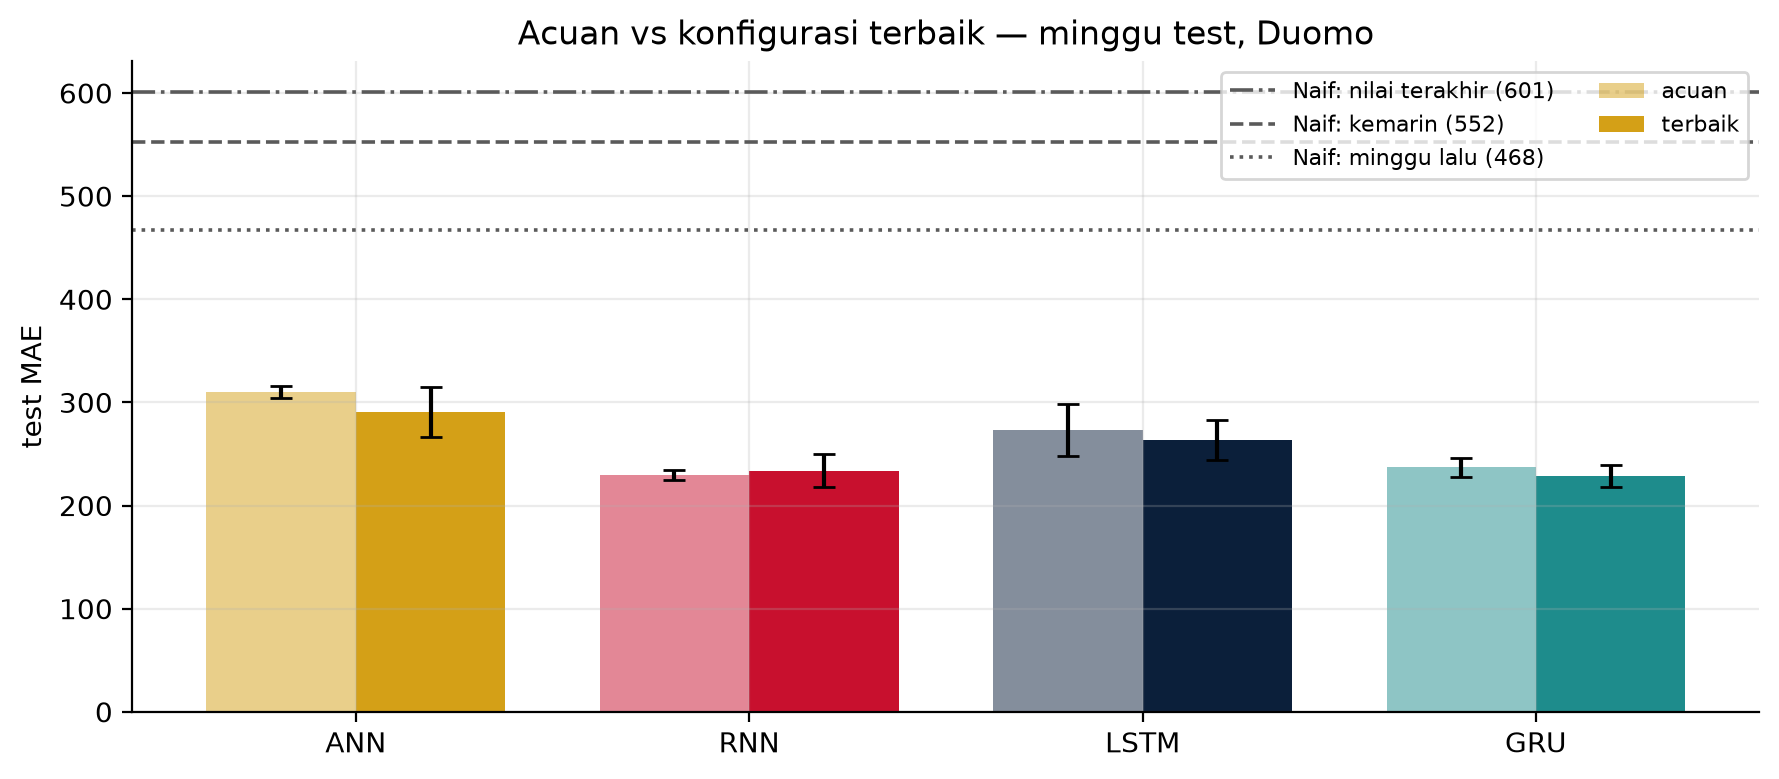
\includegraphics[width=0.95\linewidth]{C_terbaik_vs_acuan.png}
  \caption{Test MAE acuan dan konfigurasi terbaik di Duomo, dengan garis baseline naif.}
  \label{fig:c}
\end{figure}

\subsection{Uji Generalisasi}
Tabel~\ref{tab:linate} memuat baseline naif, hasil acuan, dan hasil konfigurasi terbaik Duomo di Bandara Linate (kode 5). Skala trafik Linate jauh lebih kecil (MAE sekitar 8 dibanding sekitar 230 di Duomo), sehingga galat relatif lebih layak dibandingkan: test MAPE acuan di Linate $8{,}4$--$10{,}3\,\%$ dan di Duomo $8{,}0$--$11{,}3\,\%$, sebanding.

\textbf{Urutan model.} Pada acuan, RNN dan GRU terbaik (test MAE $7{,}5$), disusul LSTM ($8{,}2$) dan ANN ($8{,}8$). Urutan ini sama dengan di Duomo (RNN, GRU, LSTM, ANN), tetapi jarak antar model menyempit: ANN lebih buruk daripada RNN sebesar $35\,\%$ di Duomo dan hanya $17\,\%$ di Linate. Setelah konfigurasi terbaik dipakai, \petunjuk{tulis urutan model dengan konfigurasi terbaik dari kolom Test Tabel~\ref{tab:linate}, lalu nyatakan apakah urutannya berubah}.

\textbf{Apakah konfigurasi terbaik Duomo tetap unggul?} \petunjuk{Bandingkan test MAE terbaik vs acuan tiap model di Linate. Pakai aturan: selisih di dalam simpangan baku berarti tidak berbeda nyata. Sebutkan model mana yang membaik, memburuk, atau tidak berubah.}

\textbf{Baseline naif dan minggu Natal.} Semua model mengalahkan baseline naif terbaik pada minggu test ($10{,}1$ untuk ``nilai terakhir''). Pada minggu Natal, ``nilai terakhir'' ($7{,}1$) justru mengalahkan semua model acuan ($10{,}8$--$14{,}4$), sehingga pelatihan pada minggu biasa tidak memberi keunggulan pada hari libur di lokasi ini.

\textbf{Pola trafik lokasi.} \petunjuk{Jelaskan pola yang terlihat pada Gambar~\ref{fig:pola}: bandingkan Duomo dan Linate (pola harian, perbedaan akhir pekan, apa yang terjadi di minggu Natal) lalu kaitkan dengan hasil di atas.}

\begin{table}[t]
  \centering
  \caption{MAE di Bandara Linate (kode 5): baseline naif, acuan, dan konfigurasi terbaik Duomo (rata-rata $\pm$ simpangan baku, 3 seed).}
  \label{tab:linate}
  \footnotesize
  \setlength{\tabcolsep}{3pt}
  \begin{tabular}{@{}llccc@{}}
    \toprule
    Model & Konfigurasi & Val & Test & Natal \\
    \midrule
    Naif: terakhir    & -- & 10,4 & 10,1 & 7,1 \\
    Naif: kemarin     & -- & 16,7 & 20,4 & 15,2 \\
    Naif: minggu lalu & -- & 13,0 & 15,4 & 28,5 \\
    \midrule
    ANN  & acuan   & $8{,}7 \pm 0{,}0$ & $8{,}8 \pm 0{,}7$ & $14{,}4 \pm 0{,}5$ \\
         & terbaik & [..] & [..] & [..] \\
    RNN  & acuan   & $8{,}5 \pm 0{,}1$ & $7{,}5 \pm 0{,}1$ & $10{,}8 \pm 0{,}1$ \\
         & terbaik & [..] & [..] & [..] \\
    LSTM & acuan   & $9{,}3 \pm 0{,}1$ & $8{,}2 \pm 0{,}2$ & $12{,}8 \pm 0{,}8$ \\
         & terbaik & [..] & [..] & [..] \\
    GRU  & acuan   & $9{,}2 \pm 0{,}1$ & $7{,}5 \pm 0{,}2$ & $11{,}4 \pm 0{,}9$ \\
         & terbaik & [..] & [..] & [..] \\
    \bottomrule
  \end{tabular}
\end{table}

\begin{figure}[t]
  \centering
  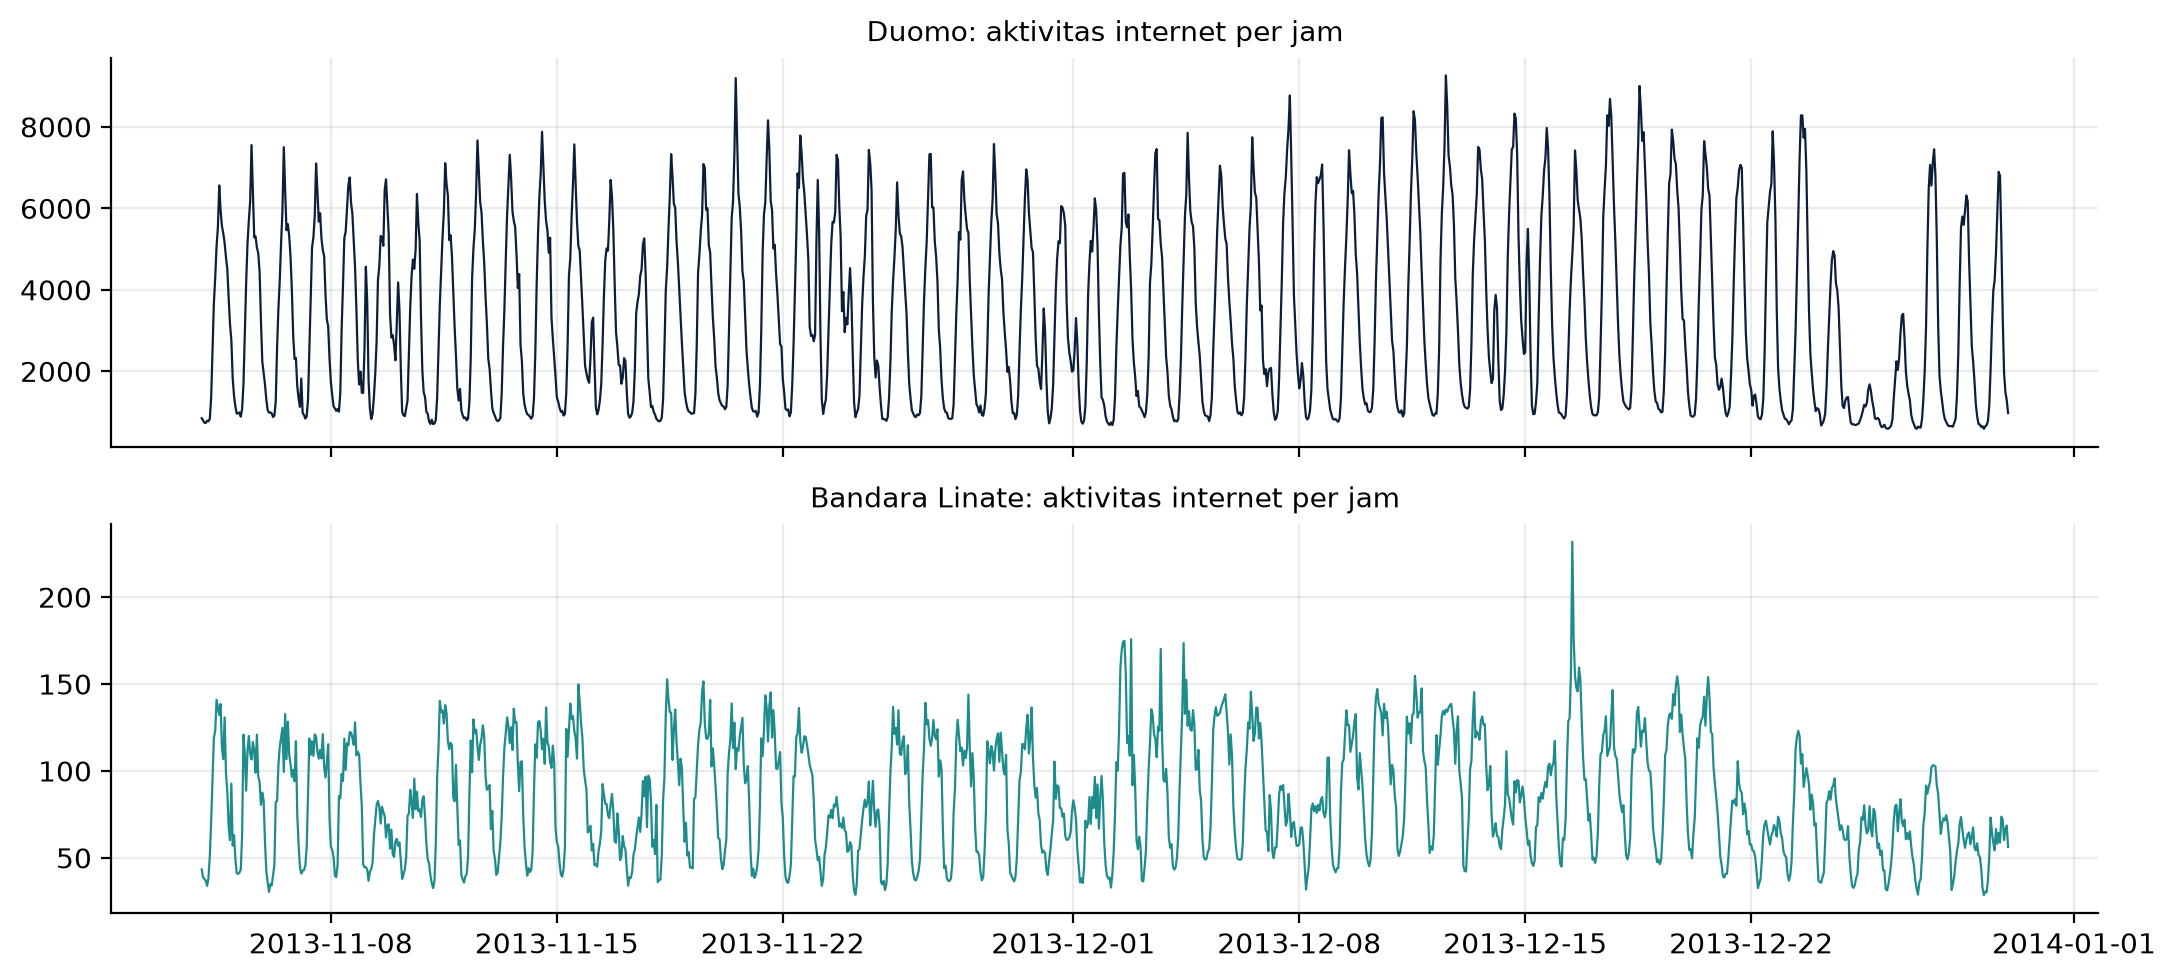
\includegraphics[width=0.95\linewidth]{D_pola_lokasi.png}
  \caption{Aktivitas internet per jam di Duomo dan Bandara Linate.}
  \label{fig:pola}
\end{figure}

% ---------------------------------------------------------------------
\section{Pembahasan}
\petunjuk{Bagian terpenting. Jangan hanya mengulang angka: jelaskan \emph{mengapa}. Hyperparameter mana yang paling berpengaruh dan mana yang tidak? Apakah perbedaan antar model lebih besar daripada perbedaan antar seed? Apa keterbatasan studi ini (satu kota, 4 minggu train, satu kali pembagian waktu)?}

% ---------------------------------------------------------------------
\section{Kesimpulan}
\petunjuk{3--5 kalimat yang menjawab pertanyaan studi, dengan angka.}

% ---------------------------------------------------------------------
\section*{Kontribusi Anggota}
\begin{tabular}{@{}lp{0.62\linewidth}@{}}
  Nama Anggota 1 & \petunjuk{contoh: Bagian A1--A3, penulisan Hasil} \\
  Nama Anggota 2 & \petunjuk{...} \\
  Nama Anggota 3 & \petunjuk{...} \\
\end{tabular}

\section*{Pernyataan Penggunaan AI}
\petunjuk{Tuliskan alat AI yang dipakai (misalnya ChatGPT, Claude, Copilot) dan untuk apa (memperbaiki kode, merapikan bahasa, dll.). Bila tidak memakai, tulis ``Tidak ada.'' Seluruh angka harus berasal dari run kalian sendiri.}

\section*{Kode dan Data}
Kode, notebook beserta output, dan seluruh hasil run tersedia di \url{https://github.com/username/nama-repo}.

\bibliographystyle{IEEEtran}
\bibliography{references}

\end{document}
